% rubber: module pdftex

\documentclass{beamer}

\usepackage[utf8]{inputenc}
\usepackage[T1]{fontenc}
\usepackage[finnish]{babel}
\usepackage{lmodern}
\usepackage{microtype}
\usepackage{amsfonts,amsmath,amssymb,amsthm}

\usepackage[fixlanguage]{babelbib}
\selectbiblanguage{finnish}

\beamertemplatenavigationsymbolsempty
\setbeamertemplate{footline}[frame number]

\usepackage{pgf,tikz}
\usepackage{tkz-euclide}
\usetikzlibrary{arrows, babel, calc, quotes}
\usetkzobj{all}

\title{Kolmiulotteinen tietokonegrafiikka ja valaistusmallinnus}
\author{Miko Mynttinen}
\date{17.4.2015}
\institute{
  Tietojenkäsittelytieteen laitos\\
  Helsingin yliopisto
}

\begin{document}
\frame{\titlepage}

\begin{frame}
\frametitle{Johdanto}
\framesubtitle{Mitä esitelmässä käsitellään}
\begin{itemize}
\item Valaistusmallinnus on tärkeä osa todenmukaisuuteen pyrkivää tietokonegrafiikkaa.
\item Kaikki näkeminen on valon heijastumista.
\item Epärealistiset valot ja varjot paljastavat helposti näkymän keinotekoisuuden.
\end{itemize}
\end{frame}

\begin{frame}
\frametitle{Johdanto}
\framesubtitle{Esitelmän rakenne}
\begin{block}{Kolmiulotteisen tietokonegrafiikan perusteet}
Miten tietokonegrafiikkaa tuotetaan?
\end{block}
\begin{block}{Phongin valaistusmalli}
Bui Tuong Phongin kehittämän valaistusmalli ja valaistusyhtälö.
\end{block}
\end{frame}
 
\begin{frame}
\frametitle{Kolmiulotteinen tietokonegrafiikka}
\begin{itemize}
\item Tietokonegrafiikka on kuvien tuottamista tietokoneella.
\item Kolmiulotteinen tietokonegrafiikka pohjautuu kolmiulotteisiin malleihin tai yhtälöihin.
\end{itemize}
\begin{figure}
\includegraphics[scale=0.3]{img/bezier.png}
\caption{Bézier-pinta.~\cite{Moller}}
\end{figure}
\end{frame}

\begin{frame}
\frametitle{Mallinnus}
\framesubtitle{Piirtoprimitiivit}
\begin{figure}
\includegraphics[scale=0.5]{img/primitives.png}
\caption{Pisteet, viivat ja kolmiot ovat piirtoprimitiivejä.}
\end{figure}
\end{frame}

\begin{frame}
\frametitle{Mallinnus}
\framesubtitle{Monikulmioverkot, yleisin tapa mallintaa kappaleita}
\begin{figure}
\includegraphics[scale=0.3]{img/sphere_wf.png}
\caption{$\sim4000$ kolmiota.}
\end{figure}
\end{frame}

\begin{frame}
\frametitle{Mallinnus}
\framesubtitle{Monikulmioverkot, yleisin tapa mallintaa kappaleita}
\begin{figure}
\includegraphics[scale=0.3]{img/dragon_wf.png}
\caption{$\sim300000$ kolmiota.}
\end{figure}
\end{frame}

\begin{frame}
\frametitle{Renderöinti}
\framesubtitle{Määritelmä}
\begin{figure}
\includegraphics[scale=0.3]{img/projection.png}
\caption{Virtuaalinen kamera.~\cite{Moller}}
\end{figure}
Renderöinti tarkoittaa kuvan tuottamista kolmiulotteisesta mallista.
\end{frame}

\begin{frame}
\frametitle{Renderöinti}
\framesubtitle{Geometriavaihe}
Geometriavaiheessa määritetään renderöitävät mallit ja projisoidaan ne kaksiulotteiselle tasolle.
\begin{itemize}
\item Mallien kääntö, skaalaus ja siirto.
\item Perspektiiviprojektio.
\item Näkymän rajaus.
\end{itemize}
\end{frame}

\begin{frame}
\frametitle{Renderöinti}
\framesubtitle{Rasterointivaihe}
Rasterointivaiheessa määritetään pikselien värit.
\begin{itemize}
\item Näkyvyyden määritys.
\item Pikseleiden värin määritys väripuskuriin.
\item Väripuskurin kopiointi näytölle tai tiedostoon.
\end{itemize}
\end{frame}

\begin{frame}
\frametitle{Phongin valaistusmalli}
\framesubtitle{Määritelmä}
\begin{block}{Valaistusmalli}
Valaistusmalli mallintaa valon käyttäytymistä.
\end{block}
\begin{block}{Phongin valaistusmallin komponentit}
\begin{itemize}
\item Ambientti valo.
\item Diffuusisti heijastunut valo.
\item Spekulaarisesti heijastunut valo.
\end{itemize}
\end{block}
\end{frame}

\begin{frame}
\frametitle{Phongin valaistusmalli}
\framesubtitle{Valon heijastuminen}
\begin{figure}
\includegraphics[scale=0.3]{img/reflections.png}
\caption{Valon heijastuminen pinnasta.~\cite{Moller}}
\end{figure}
\end{frame}

\begin{frame}
\frametitle{Phongin valaistusmalli}
\framesubtitle{Ambientti valo}
Mallintaa valon heijastumista pintojen välillä.
\begin{figure}
\includegraphics[scale=0.3]{img/sphere_ambient.png}
\caption{Pelkkä ambientti valo.}
\end{figure}
\end{frame}

\begin{frame}
\frametitle{Phongin valaistusmalli}
\framesubtitle{Diffuusisti heijastunut valo}
Mallintaa kaikkiin suuntiin heijastunutta valoa.
\begin{figure}
\includegraphics[scale=0.3]{img/sphere_ambient_diffuse.png}
\caption{Ambientti ja diffuusisti heijastunut valo.}
\end{figure}
\end{frame}

\begin{frame}
\frametitle{Phongin valaistusmalli}
\framesubtitle{Spekulaarisesti heijastunut valo}
Mallintaa näkymän katsojan suuntaan heijastunutta valoa.
\begin{figure}
\includegraphics[scale=0.3]{img/sphere_ambient_diffuse_specular.png}
\caption{Ambientti, diffuusisti ja spekulaarisesti heijastunut valo.}
\end{figure}
\end{frame}

\begin{frame}
\frametitle{Phongin valaistusmalli}
\framesubtitle{Valaistusyhtälö}
\begin{block}{Valaistusyhtälö}
Valaistusyhtälö määrittää pinnan pisteeseen osuvan valon voimakkuuden.
\end{block}
\begin{block}{Phongin valaistusyhtälö}
$I_t = \text{ambientti termi}+ \text{diffuusi termi} + \text{spekulaari termi}$.
\end{block}
\end{frame}

\begin{frame}
\frametitle{Phongin valaistusmalli}
\framesubtitle{Valaistusyhtälö}
\begin{block}{Ambientti termi}
$I_a = k_dI_p$, missä
$k_d$ on pinnan diffuusin heijastumisen kerroin ja $I_p$ pintaan osuvan valon voimakkuus.
\end{block}
\end{frame}

\begin{frame}
\frametitle{Phongin valaistusmalli}
\framesubtitle{Valaistusyhtälö}
\begin{block}{Diffuusi termi}
$I_d = k_dI_p\vec{N}\cdot\vec{L}$, missä $k_d$ on pinnan diffuusin heijastumisen kerroin ja $I_p$ pintaan osuvan valon voimakkuus.
\end{block}
\begin{figure}
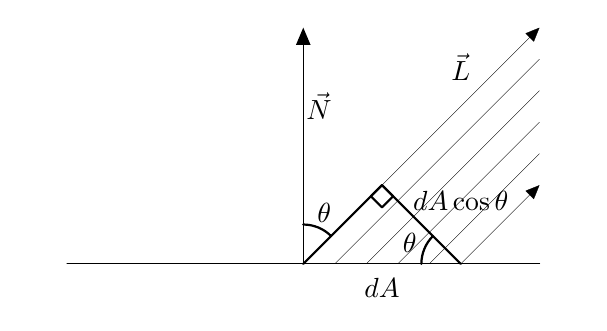
\begin{tikzpicture}[line cap=round,line join=round,>=triangle 45,x=1.0cm,y=1.0cm]
\clip(-3.5, -0.5) rectangle (3.5, 3.0);

\coordinate (O) at (0,0);
\coordinate (N) at (0, 3);

\coordinate (A) at (1, 1);
\coordinate (B) at (2, 0);
\coordinate (C) at (0, 2);

\draw [->] (O) -- (N);

\draw [->, ultra thin] (0, 0) -- (3, 3);
\draw [-, ultra thin] (0.4, 0) -- (3, 2.6);
\draw [-, ultra thin] (0.8, 0) -- (3, 2.2);
\draw [-, ultra thin] (1.2, 0) -- (3, 1.8);
\draw [-, ultra thin] (1.6, 0) -- (3, 1.4);
\draw [->, ultra thin] (2, 0) -- (3, 1);

\draw [-, thick] (A) -- (B);
\draw [-, thick] (A) -- (O);
\draw [-] (-3, 0) -- (3, 0);

\tkzMarkAngle[thick, size=0.5](A,B,O)
\tkzLabelAngle[pos=0.7](A,B,O){$\theta$}

\tkzMarkAngle[thick, size=0.5](A,O,C)
\tkzLabelAngle[pos=0.7](A,O,C){$\theta$}

\tkzMarkRightAngle[thick, size=0.2](O,A,B)

\begin{normalsize}
\draw[color=black] (2.0, 2.5) node {$\vec{L}$};
\draw[color=black] (0.2, 2.0) node {$\vec{N}$};
\draw[color=black] (1.0, -0.3) node {$dA$};
\draw[color=black] (2.0, 0.8) node {$dA\cos\theta$};
\end{normalsize}

\end{tikzpicture}
\caption{Lambertin kosinilaki.}
\end{figure}
\end{frame}

\begin{frame}
\frametitle{Phongin valaistusmalli}
\framesubtitle{Valaistusyhtälö}
\begin{block}{Spekulaari termi}
$I_s = k_sI_p(\vec{V}\cdot\vec{R})^n$,
missä $k_s$ on pinnan spekulaarin heijastumisen kerroin, $n$ vaimennuspotenssi ja $I_p$ pintaan osuvan valon voimakkuus.
\end{block}
\begin{figure}
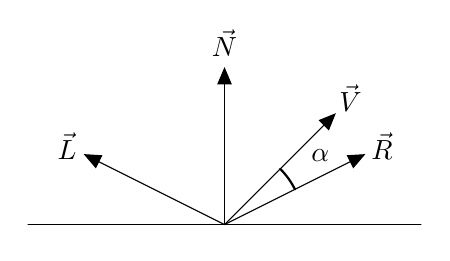
\begin{tikzpicture}[line cap=round,line join=round,>=triangle 45,x=1.0cm,y=1.0cm]
\clip(-2.5, -0.1) rectangle (2.5, 2.5);

\coordinate (O) at (0,0);
\coordinate (N) at (0, 1);
\coordinate (L) at (-3.0, 1.5);
\coordinate (V) at (2.0, 2);
\coordinate (R) at (3, 1.5);

\draw[->] (O) -- ($(O)!2cm!(R)$);
\draw[->] (O) -- ($(O)!2cm!(L)$);
\draw[->] (O) -- ($(O)!2cm!(V)$);
\draw[->] (O) -- ($(O)!2cm!(N)$);

\draw [-] (-2.5, 0) -- (2.5, 0);

\tkzMarkAngle[thick, size=1.0](R,O,V)
\tkzLabelAngle[pos=1.5](R,O,V){$\alpha$}

\begin{normalsize}
\draw[color=black] (-2.0, 1.0) node {$\vec{L}$};
\draw[color=black] (0.0, 2.3) node {$\vec{N}$};
\draw[color=black] (1.6, 1.6) node {$\vec{V}$};
\draw[color=black] (2.0, 1.0) node {$\vec{R}$};
\end{normalsize}

\end{tikzpicture}

\caption{Spekulaarisen heijastumisen suuntavektorit.}
\end{figure}
\end{frame}

\begin{frame}
\frametitle{Yhteenveto}
\begin{itemize}
\item Valaistus on tärkeää.
\item Luonto ohjaa.
\item Phongin valaistusmalli on yksinkertainen ja tehokas.
\end{itemize} 
\end{frame}

\begin{frame}
\frametitle{Loppu}
Kiitos. Kysymyksiä?
\end{frame}

\bibliographystyle{babalpha-lf}
%\bibliographystyle{babplain-lf}
\bibliography{references-fi}

\end{document}
